\section{Huffman-Codierung}

\begin{frame}
	Kann man mit einer Codierung die benötigte Anzahl der Zeichen für ein Wort reduzieren und trotzdem den Sinn erhalten?\\[0.5em]
	\pause
	Natürlich geht das (manchmal), dieses Verfahren ist überall im Einsatz:\\
	Komprimierung!
\end{frame}

\begin{frame}{Huffman-Codierung}
	Eine Huffman-Codierung ist ein präfixfreier (und demnach \enquote{einfach} zu decodierenden) Homomorphismus, bei der die Codierung eines Zeichens umso länger wird, je seltener das Zeichen vorkommt.
	
	Die Huffman-Codierung für ein Wort ist dabei nicht eindeutig, wie wir gleich im Konstruktionsverfahren sehen werden.
	
	\begin{block}{Lemma}
		Unter allen präfixfreien Codes führen Huffman-Codes zu kürzesten Codierungen
		\textbf{des Wortes, für das die Huffman-Codierung konstruiert wurde.}
	\end{block}
\end{frame}

\begin{frame}{Konstruktionsverfahren}
	Formal: In der Vorlesung\\
	Hier: Vorgehensweise (ausreichend!)
	\begin{enumerate}
		\item Für jedes Zeichen die Häufigkeit ermitteln
		\item Alle Zeichen mit ihrer Häufigkeit als Blätter in die unterste Ebene zeichnen
		\item Jeweils die zwei Knoten (nicht unbedingt Blätter!) mit den geringsten Häufigkeiten \enquote{verbinden}(also einen neuen Knoten darüber anlegen, der die Summe der Häufigkeiten erhält)
		\item Fortfahren, bis der ganze Baum aufgebaut ist.
		\item Die linken Äste mit 0 beschriften, die rechten Äste mit 1.
		\item Codierungen der Zeichen ablesen
		\item Ausgangswort codieren (wenn gefordert, vergesst das nicht!)
	\end{enumerate}
\end{frame}

\begin{frame}{Beispiel}
	Gegeben : $w= abadcadaac $ (10 Zeichen) \\[1em]
	
	\only<1-3|handout:1>{ \visible<3>{
	\begin{minipage}{0.6\linewidth}
		\begin{figure}[b]
			\centering
			\begin{tikzpicture}
			[level 1/.style={sibling distance=40mm},
			level 2/.style={sibling distance=20mm},
			level 3/.style={sibling distance=15mm}]
			\node {$10$}
			child {
				node{$5$}
				child{
					node{$3$}
					child{
						node{$1,b$}
						edge from parent node[left] {\bzero}
					}
					child {
						node{$2,d$}
						edge from parent node[right] {\bone}
					}
					edge from parent node[left] {\bzero};
				}
				child{
					node{$2,c$}
					edge from parent node[right] {\bone}
				}
				edge from parent node[left] {\bzero};
			}
			child{
				node{$5,a$}
				edge from parent node[right] {\bone}
			};
			\end{tikzpicture}
		\end{figure}  
	\end{minipage}
	}}
	\only<4-|handout:2> {
		\begin{minipage}{0.6\linewidth}
			Wie lang wird das neue Wort ?\\ \visible<5->{ 
			$5*1 + 1*3 + 2*2 + 2*3 = 18$ Zeichen\\ 
			Aber wir wollen doch komprimieren? Was haben wir falsch gemacht?\\
			\visible<6->{Nichts. Zur Codierung eines der Zeichen $a, b, c, d$ benötigen wir mindestens 2 Bit (da 4 Möglichkeiten). Für die Zeichen $0, 1$ brauchen wir aber nur ein Bit. \\
			Also haben wir 18 Bit statt 20 Bit und somit komprimiert!
		}}
		\end{minipage}
	}
	\visible<2-> {
		\begin{minipage}{0.2\linewidth}
			\hfill
			\hfill 
			\vspace*{0.1\linewidth}
			\begin{table}[H]
				\begin{tabular}{c|cccc}
					\hline
					x & a & b & c & d  \\ \hline
					$|w|_x$  & 5 & 1 & 2 & 2 \\ \hline
					h(x) & 1 & 000 & 01 & 001 \\ \hline 
				\end{tabular}
			\end{table}
		\end{minipage}
	}
\end{frame}

%TODO: Make solution frame!
\begin{frame}
		Huffman-Codierungen funktionieren immer nur gut für Wörter, die eine gleiche/ähnliche relative Zeichenhäufigkeit haben wie das Wort, für das der Code erstellt wurde.
		
		\begin{Beispiel}
			$w_1 = badcfehg, w_2 = a^1b^2c^4d^8e^{16}f^{32}g^{64}h^{128}$
			Erstellt eine Huffman-Codierung für jedes der beiden Wörter und Codiert jeweils beide Wörter mit der erstellten Codierung.\\
			Wie verhalten sich die Längen der Codewörter?
		\end{Beispiel}
\end{frame}

\begin{frame}
	\begin{block}{Erweiterung}
		Wir können nicht nur einzelne Buchstaben codieren. \\
		Bei $ w = a^{10}b^{10}c^{10} $ lohnt es sich pro Block gleicher Buchstaben eine Codierung zu haben.
	\end{block}
\end{frame}


\subsection{Aufgaben}
\begin{frame}{Aufgabe (WS 2008) }
	Das Wort $$w = \mathbf{0000\only<3->{\text{ } }0001\only<3->{\text{ } }0011\only<3->{\text{ } }0001\only<3->{\text{ } }0011\only<3->{\text{ } }0000\only<3->{\text{ } }0000\only<3->{\text{ } }1110\only<3->{\text{ } }0001\only<3->{\text{ } }0000}$$ soll komprimiert werden.
	
	\pause
	\begin{itemize}[<+->]
		\item Zerlegen Sie $w$ in Viererblöcke und bestimmen Sie die Häufigkeiten der vorkommenden Blöcke.
		\item Zur Kompression soll ein Huffman-Code verwendet werden. Benutzen Sie die in Teilaufgabe a) bestimmten Häufigkeiten, um den entsprechenden Baum aufzustellen. Beschriften Sie alle Knoten und Kanten.
		\item Geben Sie die Codierung des Wortes $w$ mit Ihrem Code an.
	\end{itemize}
\end{frame}

\begin{frame}{Lösung}
	$$w = \mathbf{0000000100110001001100000000111000010000}$$
	\textit{Zerlegen Sie $w$ in Viererblöcke und bestimmen Sie die Häufigkeiten der vorkommenden Blöcke.} \\[1em]
	\pause
	$$w = \mathbf{0000 \ 0001 \ 0011 \ 0001 \ 0011 \ 0000 \ 0000 \ 1110 \ 0001 \ 0000}$$ \pause
	\begin{table}[h!]
		\centering
		\begin{tabular}{l|cccc}	
			& 0000 & 0001 & 0011 & 1110 \\ \hline
			Absolute Häufigkeiten: & 4 & 3 & 2 & 1 \\
			Relative Häufigkeiten:  & 0,4 & 0,3 & 0,2 & 0,1\\
		\end{tabular}
	\end{table}
\end{frame}

\begin{frame}{Lösung}
	\vspace*{1em}
	\begin{minipage}{0.45\linewidth}
		\textit{Zur Kompression soll ein Huffman-Code verwendet werden. Benutzen Sie die in Teilaufgabe a) bestimmten Häufigkeiten, um den entsprechenden Baum aufzustellen. Beschriften Sie alle Knoten und Kanten.}
		\pause 
		\begin{table}[h!]
			\centering
			\begin{tabular}{cccc}	
				0000 & 0001 & 0011 & 1110 \\ \hline
				4 & 3 & 2 & 1 \\	
			\end{tabular}
		\end{table}
	\end{minipage}
	\hfill
	\begin{minipage}{0.5\linewidth}
		\begin{figure}[h!]
			\centering
			\only<3>{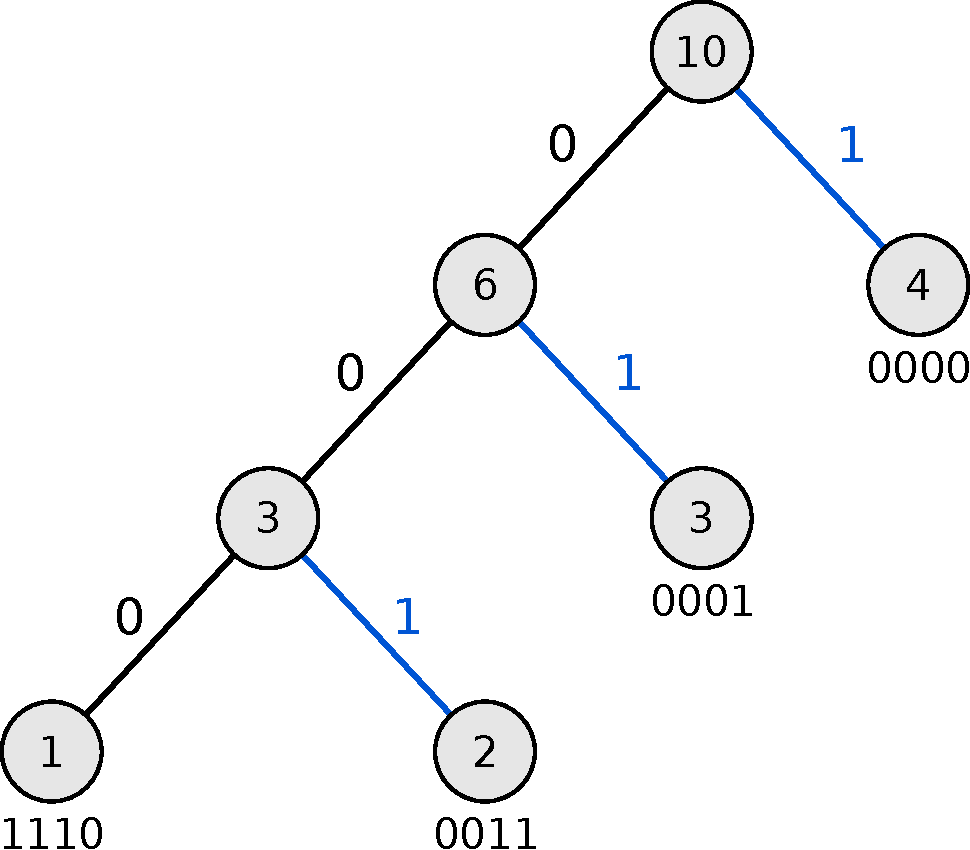
\includegraphics[scale=0.35]{Huffman.pdf}}
		\end{figure}
	\end{minipage}
\end{frame}

\begin{frame}{Lösung}
	\textit{Geben Sie die Codierung des Wortes $w$ mit Ihrem Code an.} \\[2em] \pause
	$0000000100110001001100000000111000010000$ \\ \hfill $\to 1010010100111000011$
\end{frame}

%\begin{frame}
%	\frametitle{Aufgabe (WS 2010)}
%	Seien $n, k \in \N_0$ mit $1 \leq k \leq n$. In einem Wort $w \in \{a, b, c\}^\ast$ der Länge $3n$ komme $k$ mal das Zeichen $a$, $n$ mal das Zeichen $b$ und $2n - k$ mal das Zeichen $c$ vor.
%	\begin{itemize}
%		\item Geben Sie den für die Huffman-Codierung benötigten Baum an.
%		\item Geben Sie (in Abhängigkeit von $k$ und $n$) die Länge des zu $w$ gehörenden Huffman-Codes an.
%	\end{itemize}
%\end{frame}
%
%\begin{frame}
%	\frametitle{Lösung}
%	\vspace*{1em}
%	\begin{minipage}{0.45\linewidth}
%		\textit{$\dots$ Länge $3n$ komme $k$ mal das Zeichen $a$, $n$ mal das Zeichen $b$ und $2n - k$ mal das Zeichen $c$ vor. \\[1em] Geben Sie den für die Huffman-Codierung benötigten Baum an.} 
%		\pause
%		\begin{table}[h!]
%			\centering
%			\begin{tabular}{ccc}	
%				$a$ & $b$ & $c$ \\ \hline
%				$k$ & $n$ & $2n-k$ \\	
%			\end{tabular}
%		\end{table}
%		\pause
%		$$k \leq n \leq 2n -k $$ $$ n+k+2n-k = 3n$$
%	\end{minipage}
%	\hfill
%	\begin{minipage}{0.5\linewidth}
%		\begin{figure}[h!]
%			\centering
%			\only<4>{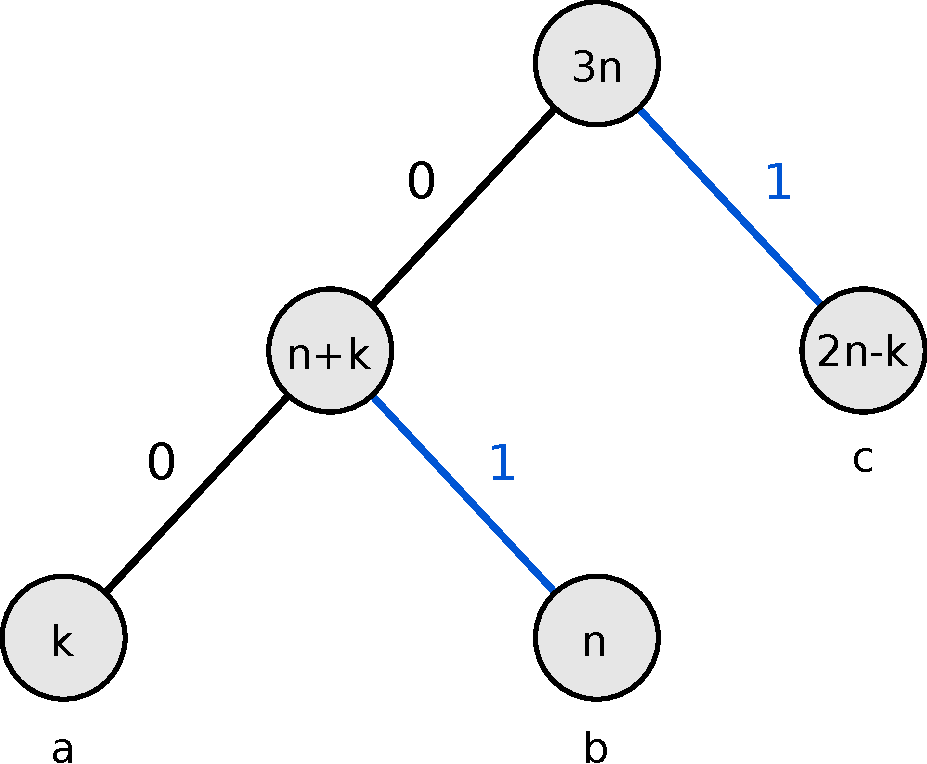
\includegraphics[scale=0.35]{Huffman2.pdf}}
%		\end{figure}
%	\end{minipage}
%\end{frame}
%
%\begin{frame}
%	\frametitle{Lösung}
%	\textit{Geben Sie die Länge des zu $w$ gehörenden Huffman-Codes an.} \\[2em]
%	\pause
%	Jedes $a$ und jedes $b$ wird durch zwei Zeichen codiert, und jedes $c$ wird durch ein Zeichen codiert. Damit erhält man insgesamt $$2k + 2n + 2n - k = 4n + k$$ Zeichen in der Codierung.
%\end{frame}


\begin{frame}{Ausblick}
	Die Huffman-Codierung hat ein Problem: Zum Decodieren muss der Huffman-Baum, der für die Codierung verwendet wurde, bekannt sein. Im wesentlichen gibt es dafür zwei Möglichkeiten:
	\begin{enumerate}
		\item Der Codebaum wird vor dem eigentlichen Codewort angegeben.\\ 
		Problem: Das verlängert das Codewort.
		\item Es wird ein vorher festgelegter Codebaum verwendet.\\
		 Problem: Dieser Codebaum ist nicht an das spezifische Wort angepasst und kann evtl. (bei komplett anderer Zeichenhäufigkeit) zu sehr schlechten Ergebnissen führen.
	\end{enumerate}

	Diese Probleme können durch andere Codierungsverfahren gelöst werden, indem z.B. das Wörterbuch dynamisch während der Decodierung aus dem Codewort aufgebaut wird (z.B. Lempel-Ziv-Welch-Verfahren).
\end{frame}

